\section{图}

\subsection{图的基本概念}

\begin{mydef}{图的定义}{graph-def}
图 $G=(V,E)$ 由顶点集 $V$ 和边集 $E$ 组成。$|V|=n$ 为顶点数（阶），$|E|=e$ 为边数。
\begin{itemize}
    \item \textbf{有向图}：边为有向边（弧）$\langle u,v\rangle$，$u$ 为弧尾，$v$ 为弧头。
    \item \textbf{无向图}：边为无向边 $(u,v)$。
    \item \textbf{简单图}：无自环（顶点到自身的边），无重边。
    \item \textbf{完全图}：无向完全图 $K_n$ 有 $\frac{n(n-1)}{2}$ 条边；有向完全图有 $n(n-1)$ 条弧。
    \item \textbf{连通}：无向图中若 $u$ 到 $v$ 有路径，称 $u,v$ 连通。若任意两顶点连通，称图为连通图。
    \item \textbf{强连通}：有向图中任意两顶点互达，称为强连通图。
\end{itemize}
\end{mydef}

\begin{conclusion}{图的基本术语速查}{graph-terms}
\begin{tablebox}{图论术语}
\centering
\begin{tabular}{|l|l|}
\hline
术语 & 含义 \\
\hline
度 $\deg(v)$ & 无向图中与 $v$ 关联的边数；$\sum\deg(v)=2e$ \\
入度 $\mathrm{id}(v)$、出度 $\mathrm{od}(v)$ & 有向图中以 $v$ 为弧头/弧尾的弧数；$\sum\mathrm{id}=\sum\mathrm{od}=e$ \\
路径 & 顶点序列，相邻顶点间有边 \\
简单路径 & 顶点不重复的路径 \\
回路（环）& 起点=终点的路径，长度 $\geq 1$ \\
连通分量 & 无向图的极大连通子图 \\
强连通分量 & 有向图的极大强连通子图 \\
生成树 & 连通图的极小连通子图，含全部 $n$ 个顶点和 $n-1$ 条边 \\
生成森林 & 非连通图中各连通分量的生成树的并 \\
\hline
\end{tabular}
\end{tablebox}
\end{conclusion}

\subsection{图的存储结构}

\begin{formula}{邻接矩阵}{adj-matrix}
用 $n\times n$ 矩阵 $A$ 表示图：
\[
A[i][j]=\begin{cases}
1 & (v_i,v_j)\text{ 或 }\langle v_i,v_j\rangle\in E\\
0 & \text{否则}
\end{cases}
\]
带权图可将 $1$ 替换为权值 $w_{ij}$，无边的位置填 $0$ 或 $\infty$。

\begin{lstlisting}[language=C]
#define MaxV 100
typedef char VType;               // 顶点类型
typedef int  EType;               // 边上权值类型
typedef struct {
    EType edges[MaxV][MaxV];      // 邻接矩阵
    VType vexs[MaxV];             // 顶点信息
    int n, e;                     // 顶点数、边数
} MGraph;
\end{lstlisting}

\textbf{特点：}
\begin{itemize}
    \item 无向图的邻接矩阵对称；有向图不一定。
    \item 空间复杂度 $O(n^2)$，适合稠密图（$e\approx n^2$）。
    \item 判断 $(v_i,v_j)$ 是否有边仅需 $O(1)$。
    \item 求顶点的度：无向图需扫描整行 $O(n)$；有向图出度扫描行、入度扫描列。
\end{itemize}
\end{formula}

\begin{formula}{邻接表}{adj-list}
为每个顶点建立一条单链表，链接其所有邻接点。

\begin{lstlisting}[language=C]
typedef struct ArcNode {
    int adjvex;                   // 邻接点下标
    EType weight;                 // 边权值（可选）
    struct ArcNode *next;         // 下一条边
} ArcNode;

typedef struct {
    VType data;                   // 顶点信息
    ArcNode *first;               // 第一条边
} VNode;

typedef struct {
    VNode adjlist[MaxV];
    int n, e;
} ALGraph;
\end{lstlisting}

\textbf{特点：}
\begin{itemize}
    \item 空间复杂度 $O(n+e)$，适合稀疏图。
    \item 无向图每条边存两次（在两个顶点的链表中各出现一次）。
    \item 求有向图出度：遍历该顶点的链表；求入度：需遍历全表或另建逆邻接表。
    \item 判断 $(v_i,v_j)$ 是否有边：需遍历 $v_i$ 的链表 $O(\deg(v_i))$。
\end{itemize}
\end{formula}

\begin{conclusion}{邻接矩阵 vs 邻接表（408 常考）}{adj-compare}
\begin{tablebox}{存储方式对比}
\centering
\begin{tabular}{|l|c|c|}
\hline
操作 & 邻接矩阵 & 邻接表 \\
\hline
空间 & $O(n^2)$ & $O(n+e)$ \\
判断 $(u,v)$ 是否有边 & $O(1)$ & $O(\deg(u))$ \\
遍历某顶点的所有邻接边 & $O(n)$ & $O(\deg(u))$ \\
适合场景 & 稠密图 & 稀疏图 \\
唯一性 & 唯一 & 不唯一（链表插入顺序可变）\\
\hline
\end{tabular}
\end{tablebox}
\end{conclusion}

\subsection{图的遍历}

\begin{conclusion}{深度优先搜索（DFS）}{dfs}
从顶点 $v$ 出发，沿一条路径走到尽头，回溯后再走其他分支。本质是递归/栈的过程。

\begin{lstlisting}[language=C]
bool visited[MaxV];
void DFS(ALGraph *G, int v) {
    visited[v] = true;
    // visit(G->adjlist[v]);    // 访问顶点 v
    for (ArcNode *p = G->adjlist[v].first; p; p = p->next)
        if (!visited[p->adjvex])
            DFS(G, p->adjvex);
}
\end{lstlisting}

邻接表表示时，DFS 时间复杂度 $O(n+e)$；邻接矩阵表示时 $O(n^2)$。

\textbf{DFS 生成树/森林：}递归过程中经过的边构成生成树（连通时）或生成森林（不连通时）。回边（back edge）是 DFS 树中指向祖先的边。
\end{conclusion}

\begin{conclusion}{广度优先搜索（BFS）}{bfs}
从顶点 $v$ 出发，逐层访问。需要辅助队列。

\begin{lstlisting}[language=C]
void BFS(ALGraph *G, int v) {
    int queue[MaxV], front = 0, rear = 0;
    visited[v] = true;
    queue[rear++] = v;
    while (front < rear) {
        int u = queue[front++];
        // visit(G->adjlist[u]);
        for (ArcNode *p = G->adjlist[u].first; p; p = p->next)
            if (!visited[p->adjvex]) {
                visited[p->adjvex] = true;
                queue[rear++] = p->adjvex;
            }
    }
}
\end{lstlisting}

邻接表 $O(n+e)$，邻接矩阵 $O(n^2)$。

\textbf{BFS 生成树：}BFS 过程中首次发现某顶点所用的边构成生成树。BFS 生成树中从根到任意顶点的路径即最短路径（边数最少）。
\end{conclusion}

\begin{attention}
\textbf{408 常考：DFS/BFS 遍历序列的唯一性。}邻接矩阵表示的图遍历序列唯一（因为邻接点按顶点编号有序）；邻接表表示的图遍历序列不唯一（取决于链表插入顺序）。
\end{attention}

\subsection{最小生成树（MST）}

\begin{mydef}{最小生成树}{mst}
连通带权无向图的生成树中，边权值和最小者称为最小生成树（Minimum Spanning Tree）。MST 可能不唯一，但边权和唯一。
\end{mydef}

\begin{conclusion}{Prim 算法}{prim}
从某一顶点开始，每次选一条连接「已在树中顶点」和「不在树中顶点」的最小权边，将对应顶点加入树。重复 $n-1$ 次。

\begin{lstlisting}[language=C]
// Prim — O(n^2) 实现（邻接矩阵，适合稠密图）
void Prim(MGraph G, int start) {
    int lowcost[MaxV];      // lowcost[i]: i到当前MST的最小边权
    int closest[MaxV];      // closest[i]: MST中与i最近的顶点
    bool inTree[MaxV] = {false};
    inTree[start] = true;
    for (int i = 0; i < G.n; i++) {
        lowcost[i] = G.edges[start][i];
        closest[i] = start;
    }
    for (int k = 1; k < G.n; k++) {
        int min = INF, u = -1;
        for (int i = 0; i < G.n; i++)
            if (!inTree[i] && lowcost[i] < min)
                { min = lowcost[i]; u = i; }
        inTree[u] = true;
        // 输出边 (closest[u], u) 权 min
        for (int i = 0; i < G.n; i++)
            if (!inTree[i] && G.edges[u][i] < lowcost[i])
                { lowcost[i] = G.edges[u][i]; closest[i] = u; }
    }
}
\end{lstlisting}
时间复杂度 $O(n^2)$，与边数无关——适合稠密图。用堆优化可达 $O(e\log n)$。
\end{conclusion}

\begin{conclusion}{Kruskal 算法}{kruskal}
按边权从小到大依次选边，若该边连接两个不同连通分量则加入 MST，否则丢弃。直到选出 $n-1$ 条边。

时间复杂度 $O(e\log e)$（排序主导），适合稀疏图。需用并查集维护连通分量。
\end{conclusion}

\begin{attention}
408 选择题常考：给定一个图，手动执行 Prim（指定起点）或 Kruskal 得到 MST。注意当有多条等权边时 MST 可能不唯一，但权值和唯一。
\end{attention}

\subsection{最短路径}

\begin{conclusion}{Dijkstra 算法}{dijkstra}
求\textbf{单源最短路径}（非负权值）。类似 Prim，贪心思想：

\begin{lstlisting}[language=C]
void Dijkstra(MGraph G, int s, int dist[], int path[]) {
    bool final[MaxV] = {false};
    for (int i = 0; i < G.n; i++) {
        dist[i] = G.edges[s][i];
        path[i] = (dist[i] < INF) ? s : -1;
    }
    final[s] = true; dist[s] = 0;
    for (int k = 1; k < G.n; k++) {
        int min = INF, u = -1;
        for (int i = 0; i < G.n; i++)
            if (!final[i] && dist[i] < min)
                { min = dist[i]; u = i; }
        final[u] = true;
        for (int i = 0; i < G.n; i++)
            if (!final[i] && dist[u] + G.edges[u][i] < dist[i])
                { dist[i] = dist[u] + G.edges[u][i]; path[i] = u; }
    }
}
\end{lstlisting}
时间复杂度 $O(n^2)$（邻接矩阵），堆优化可达 $O(e\log n)$。

\textbf{与 Prim 的关键区别：}Prim 的 \texttt{lowcost[i]} 是顶点 $i$ 到当前 MST 集合的\textbf{最小边权}；Dijkstra 的 \texttt{dist[i]} 是源点到顶点 $i$ 的\textbf{累计路径长度}。两者代码结构相似，更新条件不同。
\end{conclusion}

\begin{conclusion}{Floyd 算法}{floyd}
求\textbf{所有顶点对}间的最短路径。DP 思想：依次考虑以每个顶点为中间点时能否缩短路径。

\begin{lstlisting}[language=C]
void Floyd(MGraph G, int D[][MaxV], int path[][MaxV]) {
    for (int i = 0; i < G.n; i++)
        for (int j = 0; j < G.n; j++) {
            D[i][j] = G.edges[i][j];
            path[i][j] = (D[i][j] < INF && i != j) ? i : -1;
        }
    for (int k = 0; k < G.n; k++)
        for (int i = 0; i < G.n; i++)
            for (int j = 0; j < G.n; j++)
                if (D[i][k] + D[k][j] < D[i][j]) {
                    D[i][j] = D[i][k] + D[k][j];
                    path[i][j] = path[k][j];
                }
}
\end{lstlisting}
时间复杂度 $O(n^3)$。允许负权边，但不能有负权回路。
\end{conclusion}

\begin{attention}
\textbf{408 高频考点：}Dijkstra 算法中若存在负权边则失效（已确定最短的顶点可能在后续被更新）。Floyd 允许负权边但要求无负权回路。
\end{attention}

\subsection{有向无环图（DAG）与拓扑排序}

\begin{mydef}{拓扑排序}{topo-sort}
将有向无环图（DAG）的所有顶点排成一个线性序列，使得对每条弧 $\langle u,v\rangle$，$u$ 在序列中出现在 $v$ 之前。拓扑序列不唯一。
\end{mydef}

\begin{conclusion}{拓扑排序算法}{topo-algo}
基于入度：每次选一个入度为 $0$ 的顶点输出并将其所有出边的终点入度减 $1$。重复直到所有顶点输出（成功）或不存在入度 $0$ 的顶点（有回路）。

\begin{lstlisting}[language=C]
bool TopoSort(ALGraph *G, int topo[]) {
    int indegree[MaxV] = {0}, cnt = 0;
    int stack[MaxV], top = -1;
    for (int i = 0; i < G->n; i++)          // 计算入度
        for (ArcNode *p = G->adjlist[i].first; p; p = p->next)
            indegree[p->adjvex]++;
    for (int i = 0; i < G->n; i++)          // 入度为0入栈
        if (indegree[i] == 0) stack[++top] = i;
    while (top != -1) {
        int u = stack[top--];
        topo[cnt++] = u;
        for (ArcNode *p = G->adjlist[u].first; p; p = p->next) {
            int v = p->adjvex;
            if (--indegree[v] == 0) stack[++top] = v;
        }
    }
    return cnt == G->n;                     // cnt<n 则有回路
}
\end{lstlisting}
时间复杂度 $O(n+e)$。用栈或队列均可——用栈得到逆拓扑序更自然（DFS 的逆后序即拓扑序）。
\end{conclusion}

\subsection{AOE 网与关键路径}

\begin{mydef}{AOV 网与 AOE 网}{aov-aoe}
\begin{itemize}
    \item \textbf{AOV 网}（Activity On Vertex）：顶点表示活动，边表示活动间的优先关系。
    \item \textbf{AOE 网}（Activity On Edge）：边表示活动，边权表示活动持续时间；顶点表示事件（某些活动完成的时刻）。
\end{itemize}
\end{mydef}

\begin{conclusion}{关键路径}{critical-path}
AOE 网中：
\begin{itemize}
    \item \textbf{事件 $v_k$ 的最早发生时间 $ve(k)$}：从源点到 $v_k$ 的最长路径长度。按拓扑序计算：$ve(k)=\max\{ve(j)+\mathrm{weight}(\langle v_j,v_k\rangle)\}$。
    \item \textbf{事件 $v_k$ 的最迟发生时间 $vl(k)$}：不推迟工期的前提下事件最迟发生时间。按逆拓扑序计算：$vl(k)=\min\{vl(j)-\mathrm{weight}(\langle v_k,v_j\rangle)\}$，汇点 $vl=ve$。
    \item \textbf{活动 $a_i=\langle v_j,v_k\rangle$ 的最早开始 $e(i)=ve(j)$}，\textbf{最迟开始 $l(i)=vl(k)-\mathrm{weight}$}。
    \item \textbf{关键活动}：$e(i)=l(i)$ 的活动。\textbf{关键路径}：由关键活动构成的从源点到汇点的路径。
\end{itemize}

\textbf{408 常考：}给定 AOE 网，计算各事件的 $ve$ 和 $vl$，找出关键活动和关键路径。关键路径可能不唯一——缩短某条关键路径上的非公共关键活动不一定会缩短总工期。
\end{conclusion}

\subsection{408 高频考点速查}

\begin{conclusion}{图 — 408 选择题常考点}{graph-408-keypoints}
\begin{enumerate}
    \item \textbf{连通图边数范围}：$n-1\leqslant e \leqslant C_n^2$（最少 $n-1$ 即生成树）。
    \item \textbf{DFS/BFS 遍历序列}：邻接矩阵唯一，邻接表不唯一。
    \item \textbf{Prim vs Kruskal}：稠密图用 Prim $O(n^2)$，稀疏图用 Kruskal $O(e\log e)$。
    \item \textbf{Dijkstra 适用条件}：非负权值；与 Prim 代码对比。
    \item \textbf{拓扑排序}：DAG 才有拓扑序列；不唯一的条件（有多个人度同时为 0 的顶点）。
    \item \textbf{关键路径}：$ve$ 和 $vl$ 的计算；关键活动 $e=l$；缩短非关键活动不缩短工期。
    \item \textbf{不同存储结构的遍历复杂度}：邻接表 $O(n+e)$ vs 邻接矩阵 $O(n^2)$。
\end{enumerate}
\end{conclusion}

\newpage
\section{习题}

\subsection{基础过关题}

\begin{enumerate}

\item \textbf{（单项选择题）} 具有 $n$ 个顶点的无向完全图有边数为
\begin{center}
\begin{tabular}{ll}
(A) $n(n-1)$ & (B) $\dfrac{n(n-1)}{2}$ \\[6pt]
(C) $n^2$ & (D) $\dfrac{n^2}{2}$
\end{tabular}
\end{center}

\item \textbf{（单项选择题）} 对于一个具有 $n$ 个顶点和 $e$ 条边的无向图，若用邻接表存储，则所有顶点的边链表中结点总数为
\begin{center}
\begin{tabular}{ll}
(A) $e$ & (B) $2e$ \\[6pt]
(C) $e/2$ & (D) $n+e$
\end{tabular}
\end{center}

\item \textbf{（单项选择题）} 以下关于最小生成树的说法中，正确的是
\begin{center}
\begin{tabular}{ll}
(A) 最小生成树唯一 & (B) 最小生成树的边权和唯一 \\[4pt]
(C) Prim 算法适合稀疏图 & (D) Kruskal 算法适合稠密图
\end{tabular}
\end{center}

\item \textbf{（填空题）} 设有向图 $G$ 的邻接矩阵为 $A$，则 $A^k$ 的元素 $A^k[i][j]$ 表示从顶点 $i$ 到顶点 $j$ 的长度为 $k$ 的 \underline{\qquad\qquad}。

\item \textbf{（填空题）} 对下图进行深度优先遍历（从顶点 1 出发，按编号递增顺序选择邻接点），得到的 DFS 序列是 \underline{\qquad\qquad}。
\begin{center}
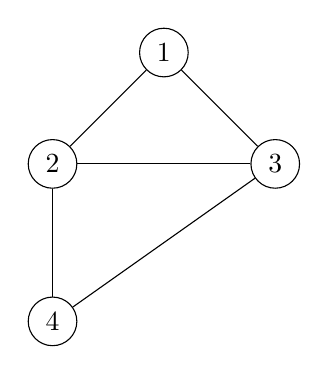
\begin{tikzpicture}[>=stealth, node distance=2cm, auto]
\node[draw, circle] (1) {1};
\node[draw, circle, below left of=1] (2) {2};
\node[draw, circle, below right of=1] (3) {3};
\node[draw, circle, below of=2] (4) {4};
\draw[-] (1) -- (2);
\draw[-] (1) -- (3);
\draw[-] (2) -- (3);
\draw[-] (2) -- (4);
\draw[-] (3) -- (4);
\end{tikzpicture}
\end{center}

\item \textbf{（简答题）} 简述 Prim 算法和 Dijkstra 算法的相似之处与本质区别。

\item \textbf{（简答题）} 已知有向图 $G$ 的边集为 $\{\langle1,2\rangle,\langle1,3\rangle,\langle2,4\rangle,\langle3,2\rangle,\langle3,5\rangle,\langle4,3\rangle,\langle4,5\rangle\}$。写出 $G$ 的一个拓扑排序序列，并说明该图是否存在回路。

\item \textbf{（算法设计）} 编写算法，判断无向图 $G$ 是否为连通图。分析时间复杂度。

\end{enumerate}

\subsection{真题风格与综合训练}

\begin{enumerate}[resume]

\item \textbf{（真题风格，单项选择题）} 以下关于图的存储结构的说法中，错误的是
\begin{center}
\begin{tabular}{ll}
(A) 邻接矩阵存储的图，DFS 遍历序列唯一 \\[4pt]
(B) 邻接表存储的图，BFS 遍历序列不唯一 \\[4pt]
(C) 邻接矩阵的空间复杂度与边数无关 \\[4pt]
(D) 邻接表存储有向图时，求顶点的入度需遍历全表
\end{tabular}
\end{center}

\item \textbf{（真题风格，单项选择题）} 用 Dijkstra 算法求下图中从顶点 1 到其余各点的最短路径，当算法选出顶点 3 之后（即顶点 3 的 dist 被最终确定时），顶点 5 的当前 dist 值为
\begin{center}
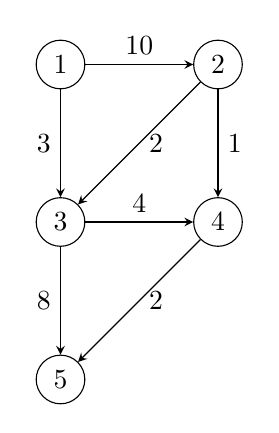
\begin{tikzpicture}[>=stealth, node distance=2cm, auto]
\node[draw, circle] (1) {1};
\node[draw, circle, right of=1] (2) {2};
\node[draw, circle, below of=1] (3) {3};
\node[draw, circle, below of=2] (4) {4};
\node[draw, circle, below of=3] (5) {5};
\draw[->] (1) -- node[above] {10} (2);
\draw[->] (1) -- node[left]  {3}  (3);
\draw[->] (2) -- node[right] {1}  (4);
\draw[->] (3) -- node[above] {4}  (4);
\draw[->] (3) -- node[left] {8}  (5);
\draw[->] (4) -- node[right] {2}  (5);
\draw[->] (2) -- node[right] {2}  (3);
\end{tikzpicture}
\end{center}
\begin{center}
\begin{tabular}{ll}
(A) $8$ & (B) $9$ \\[6pt]
(C) $10$ & (D) $11$
\end{tabular}
\end{center}

\item \textbf{（真题风格，综合题）} 某工程项目包含 8 个活动，其 AOE 网如下（边上的数字为活动持续时间）。求：
\begin{enumerate}
    \item[(1)] 各事件的最早发生时间 $ve$ 与最迟发生时间 $vl$；
    \item[(2)] 关键路径及工程总工期；
    \item[(3)] 若活动 $a_4$ 的持续时间延长 3 天，总工期如何变化？说明理由。
\end{enumerate}

\item \textbf{（真题风格，综合题）} 设带权连通无向图 $G$ 的边权互不相同。证明：$G$ 的最小生成树唯一。Kruskal 算法在此条件下是否一定得到该唯一 MST？为什么？

\item \textbf{（真题风格，综合题）} 有向图 $G=(V,E)$ 用邻接表存储。
\begin{enumerate}
    \item[(1)] 编写算法，判断 $G$ 中是否存在从顶点 $u$ 到顶点 $v$ 的长度为 $k$ 的路径（$k\geqslant0$）；
    \item[(2)] 分析算法的时间复杂度。
\end{enumerate}

\end{enumerate}

\vspace{8pt}
\noindent\textbf{拓展阅读：}
\begin{itemize}
    \item 邓俊辉《数据结构（C++语言版）》第 6 章「图」——完整的图 ADT 实现，包括 BFS/DFS、Prim/Kruskal、Dijkstra 的 C++ 代码和复杂度分析。
    \item Sedgewick《算法》第 4 章「图」——无向图/有向图的 DFS/BFS 经典讨论，第 4.3 节最小生成树，第 4.4 节最短路径。
\end{itemize}
